\documentclass{beamer}

\usepackage[utf8]{inputenc}
\usepackage[T1]{fontenc}
\usepackage{amsmath}
\usepackage{bm}
\usepackage{algorithm}
\usepackage{algpseudocode}
\usepackage{caption}
\usepackage{graphicx}
\usepackage{hyperref}
\usepackage{booktabs}
\usepackage{tikz}
\usetikzlibrary{arrows.meta, positioning, calc, fit}

\setbeamertemplate{headline}{}
\usetheme[compress]{Berlin}
\setbeamertemplate{page number in head/foot}[framenumber]
\captionsetup{justification=centering, font={scriptsize}, skip=0pt}
\graphicspath{{../../tp3-visual/graphs/}{resources/}}

\title[Filas Inteligentes]{Filas Inteligentes: Trabajo Pr\'actico Nro. 3}
\subtitle{72.25 - Simulaci\'on de Sistemas}
\author[J. Birsa, J. Gonzalez Cornet, F. Magri]{
  Juan Pablo Birsa\inst{1} \and
  Josefina Gonzalez Cornet\inst{2} \and
  Federico Jos\'e Magri\inst{3}
}
\institute[ITBA]{
  \inst{1} jbirsa@itba.edu.ar (64500) \\
  \inst{2} jgonzalezcornet@itba.edu.ar (64550) \\
  \inst{3} fmagri@itba.edu.ar (64508) \\
}
\date{2026 1C | Grupo Nro. 5}

\makeatletter
\beamer@theme@subsectionfalse
\makeatother

\AtBeginSection[]{
    \begin{frame}
        \begin{beamercolorbox}[sep=8pt,center]{title}
            \usebeamerfont{title}\insertsection
        \end{beamercolorbox}
    \end{frame}
}

\newcommand{\resultpair}[5]{%
    \begin{minipage}[t]{0.48\textwidth}
        \centering
        \parbox[c][0.08\textheight][c]{\textwidth}{\centering\small #1}
        \\
        \includegraphics[width=\textwidth,height=0.40\textheight,keepaspectratio]{#2}
    \end{minipage}
    \hfill
    \begin{minipage}[t]{0.48\textwidth}
        \centering
        \parbox[c][0.08\textheight][c]{\textwidth}{\centering\small #3}
        \\
        \includegraphics[width=\textwidth,height=0.40\textheight,keepaspectratio]{#4}
    \end{minipage}

    \vspace{0.05cm}
    \begin{beamercolorbox}[sep=4pt,center]{block body}
        \small #5
    \end{beamercolorbox}
}

\newcommand{\paramsbox}[1]{%
    \begin{beamercolorbox}[sep=4pt,center]{block body}
        \small #1
    \end{beamercolorbox}
}

\begin{document}

\begin{frame}
  \titlepage
\end{frame}

\section{Introducci\'on}

\begin{frame}{Sistema Real}
    Los sistemas con m\'ultiples servidores y filas aparecen en:
    \begin{itemize}
        \item Cajas de supermercado y centros de atenci\'on.
        \item Check-in, embarque y controles de acceso.
        \item Peajes y otros sistemas con congesti\'on espacial.
    \end{itemize}

    \vspace{0.1cm}
    {\small Interesa comparar c\'omo la frecuencia de llegada, el tiempo de servicio y la geometr\'ia de la fila modifican la congesti\'on y la permanencia de los clientes.}

    \begin{figure}[htbp]
        \centering
        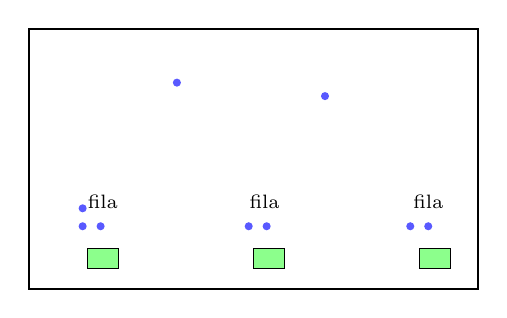
\begin{tikzpicture}[scale=0.57]
            \draw[thick] (0,0) rectangle (10,5.8);
            \foreach \x in {1.3,5,8.7} {
                \filldraw[fill=green!45, draw=black] (\x,0.45) rectangle +(0.7,0.45);
            }
            \foreach \p in {(1.2,1.4),(1.6,1.4),(1.2,1.8),(4.9,1.4),(5.3,1.4),(8.5,1.4),(8.9,1.4),(6.6,4.3),(3.3,4.6)} {
                \fill[blue!65] \p circle (0.09);
            }
            \node[font=\scriptsize] at (1.65,1.95) {fila};
            \node[font=\scriptsize] at (5.25,1.95) {fila};
            \node[font=\scriptsize] at (8.9,1.95) {fila};
        \end{tikzpicture}
    \end{figure}
\end{frame}

\begin{frame}{Modelo Matem\'atico}
    Proceso de arribo:
    \begin{equation*}
        \Delta t_{\text{arr}} \sim \mathrm{Exp}\!\left(\frac{1}{t_1}\right)
    \end{equation*}

    Proceso de servicio:
    \begin{equation*}
        \Delta t_{\text{serv}} \sim \mathrm{Exp}\!\left(\frac{1}{t_2}\right)
    \end{equation*}

    Tiempo de desplazamiento del cliente:
    \begin{equation*}
        t_{\text{cam}} = \frac{d}{v}, \qquad v = 1\,\mathrm{m/s}
    \end{equation*}

    Evoluci\'on dirigida por eventos:
    \begin{equation*}
        t_{n+1} = t_n + \min\{\Delta t_{\text{evento}}\}
    \end{equation*}
\end{frame}

\begin{frame}{Asignaci\'on Probabil\'istica}
    \begin{minipage}[t]{0.57\textwidth}
        Para cada servidor $i$ se defini\'o un costo temporal estimado:
        \begin{equation*}
            c_i = \frac{d_i}{v} + n_i\,t_2
        \end{equation*}
        donde $d_i$ es la distancia al servidor y $n_i$ la carga asociada a su fila.

        La asignaci\'on final se realiza con un sorteo ponderado:
        \begin{equation*}
            P_i = \frac{e^{-c_i}}{\sum_j e^{-c_j}}
        \end{equation*}
    \end{minipage}
    \hfill
    \begin{minipage}[t]{0.38\textwidth}
        Modalidades:
        \begin{itemize}
            \item A: una fila por servidor.
            \item B: una fila \~unica compartida.
        \end{itemize}

        Filas:
        \begin{itemize}
            \item Guiada: serpentina.
            \item Libre: heur\'istica espacial.
        \end{itemize}
    \end{minipage}
\end{frame}

\section{Implementaci\'on}

\begin{frame}{Arquitectura del Motor}
    \centering
    
\includegraphics[width=0.98\textwidth,height=0.72\textheight,keepaspectratio]{diagram.jpeg}

    \vspace{0.1cm}
    \paramsbox{El motor inicializa servidores y colas, agenda eventos y escribe el estado del sistema en cada evento.}
\end{frame}

\begin{frame}{Algoritmo Implementado}
    \begin{algorithm}[H]
    \small
        \caption{Loop principal de simulaci\'on dirigida por eventos}
        \begin{algorithmic}[1]
            \State Inicializar servidores, colas y estructura de eventos.
            \State Agendar el primer arribo de cliente.
            \While{haya eventos con $t \leq t_f$}
                \State Tomar el pr\'oximo evento de la cola prioritaria.
                \State Actualizar posiciones interpoladas de clientes en movimiento.
                \State Procesar el evento correspondiente.
                \State Registrar el largo de fila en ese instante.
                \State Escribir el snapshot del sistema en el output.
            \EndWhile
            \State Calcular observables acumulados y escribir estad\'isticas finales.
        \end{algorithmic}
    \end{algorithm}

    \vspace{0.15cm}
    \footnotesize Eventos concretos: arribo de cliente, llegada al lugar en la fila, avance en fila, llegada al servidor y fin de servicio.
\end{frame}

\begin{frame}{Tipos de Fila Implementados}
    \begin{minipage}[t]{0.48\textwidth}
        \centering
        \small Fila guiada tipo serpentina\\[0.1cm]
        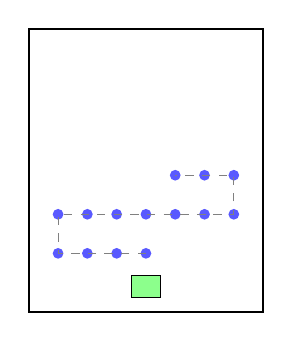
\begin{tikzpicture}[scale=0.62]
            \draw[thick] (0,0) rectangle (4.8,5.8);
            \filldraw[fill=green!45, draw=black] (2.1,0.3) rectangle +(0.6,0.45);
            \foreach \p in {(2.4,1.2),(1.8,1.2),(1.2,1.2),(0.6,1.2),(0.6,2.0),(1.2,2.0),(1.8,2.0),(2.4,2.0),(3.0,2.0),(3.6,2.0),(4.2,2.0),(4.2,2.8),(3.6,2.8),(3.0,2.8)} {
                \fill[blue!65] \p circle (0.11);
            }
            \draw[gray, dashed]
                (2.4,1.2) -- (1.8,1.2) -- (1.2,1.2) -- (0.6,1.2)
                -- (0.6,2.0) -- (1.2,2.0) -- (1.8,2.0) -- (2.4,2.0)
                -- (3.0,2.0) -- (3.6,2.0) -- (4.2,2.0)
                -- (4.2,2.8) -- (3.6,2.8) -- (3.0,2.8);
        \end{tikzpicture}
    \end{minipage}
    \hfill
    \begin{minipage}[t]{0.48\textwidth}
        \centering
        \small Fila libre en el espacio\\[0.1cm]
        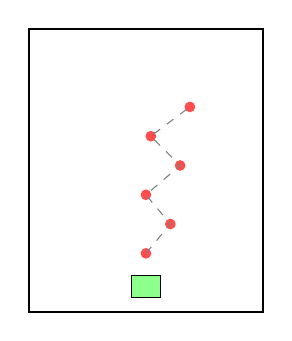
\begin{tikzpicture}[scale=0.62]
            \draw[thick] (0,0) rectangle (4.8,5.8);
            \filldraw[fill=green!45, draw=black] (2.1,0.3) rectangle +(0.6,0.45);
            \foreach \p in {(2.4,1.2),(2.9,1.8),(2.4,2.4),(3.1,3.0),(2.5,3.6),(3.3,4.2)} {
                \fill[red!70] \p circle (0.11);
            }
            \draw[gray, dashed] (2.4,1.2) -- (2.9,1.8) -- (2.4,2.4) -- (3.1,3.0) -- (2.5,3.6) -- (3.3,4.2);
        \end{tikzpicture}
    \end{minipage}

    \vspace{0.15cm}
    \paramsbox{En la fila guiada los puestos se precalculan sobre una grilla. En la fila libre los puestos se generan incrementalmente a $1\,\mathrm{m}$ del anterior, manteniendo separaci\'on y permanencia dentro del recinto.}
\end{frame}

\section{Simulaciones}

\begin{frame}{Sistema Particular}
    \begin{minipage}[t]{0.49\textwidth}
        \centering
        \small Modalidad A\\[0.1cm]
        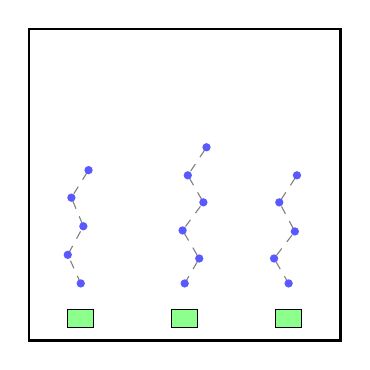
\begin{tikzpicture}[scale=0.66]
            \draw[thick] (0,0) rectangle (6,6);
            \foreach \x in {1,3,5} {
                \filldraw[fill=green!45, draw=black] (\x-0.25,0.25) rectangle +(0.5,0.35);
            }
            \draw[gray, dashed] (1.0,1.1) -- (0.75,1.65) -- (1.05,2.20) -- (0.82,2.75) -- (1.15,3.28);
            \draw[gray, dashed] (3.0,1.1) -- (3.28,1.58) -- (2.96,2.12) -- (3.36,2.66) -- (3.06,3.18) -- (3.42,3.72);
            \draw[gray, dashed] (5.0,1.1) -- (4.72,1.58) -- (5.12,2.10) -- (4.82,2.66) -- (5.16,3.18);
            \foreach \p in {(1.0,1.1),(0.75,1.65),(1.05,2.20),(0.82,2.75),(1.15,3.28),(3.0,1.1),(3.28,1.58),(2.96,2.12),(3.36,2.66),(3.06,3.18),(3.42,3.72),(5.0,1.1),(4.72,1.58),(5.12,2.10),(4.82,2.66),(5.16,3.18)} {
                \fill[blue!65] \p circle (0.08);
            }
        \end{tikzpicture}
    \end{minipage}
    \hfill
    \begin{minipage}[t]{0.49\textwidth}
        \centering
        \small Modalidad B\\[0.1cm]
        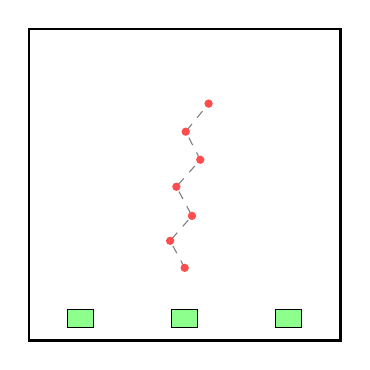
\begin{tikzpicture}[scale=0.66]
            \draw[thick] (0,0) rectangle (6,6);
            \foreach \x in {1,3,5} {
                \filldraw[fill=green!45, draw=black] (\x-0.25,0.25) rectangle +(0.5,0.35);
            }
            \draw[gray, dashed] (3.0,1.4) -- (2.72,1.92) -- (3.14,2.40) -- (2.84,2.96) -- (3.30,3.48) -- (3.02,4.02) -- (3.46,4.56);
            \foreach \p in {(3.0,1.4),(2.72,1.92),(3.14,2.40),(2.84,2.96),(3.30,3.48),(3.02,4.02),(3.46,4.56)} {
                \fill[red!70] \p circle (0.08);
            }
        \end{tikzpicture}
    \end{minipage}

    \vspace{0.15cm}
    \paramsbox{Recinto cuadrado de $30 \times 30\,\mathrm{m}^2$, servidores sobre un borde, clientes generados en posiciones aleatorias del plano y movimiento a $1\,\mathrm{m/s}$.}
\end{frame}

\begin{frame}{Par\'ametros Estudiados}
    Par\'ametros fijos del sistema:
    \begin{itemize}
        \item Recinto: $30 \times 30\,\mathrm{m}^2$.
        \item Velocidad de caminata: $1\,\mathrm{m/s}$.
        \item Llegadas Poisson y servicios exponenciales.
        \item Animaciones ilustrativas con $k=3$.
    \end{itemize}

    Barridos cuantitativos realizados sobre fila guiada tipo serpentina:
    \begin{itemize}
        \item $t_2 \in [1, 8] \;\mathrm{s}$, con $t_1 = 1\,\mathrm{s}$ y $k = 5$.
        \item $t_1 \in [0.3, 3] \;\mathrm{s}$, con $t_2 = 3\,\mathrm{s}$ y $k = 5$.
        \item $k \in [1, 8]$, con $t_1 = 1\,\mathrm{s}$ y $t_2 = 3\,\mathrm{s}$.
    \end{itemize}
\end{frame}

\begin{frame}{Observables Definidos}
    Largo total de fila:
    \begin{equation*}
        L(t) = \sum_{q=1}^{N_{\text{colas}}} \ell_q(t)
    \end{equation*}

    Promedio temporal en r\'egimen estacionario:
    \begin{equation*}
        \bar{L} = \frac{1}{t_f} \int_0^{t_f} L(t) \, dt
    \end{equation*}

    Tasa de crecimiento cuando no hay estacionario:
    \begin{equation*}
        m = \frac{dL}{dt}
    \end{equation*}

    \paramsbox{La estabilidad se eval\'ua a partir del ajuste lineal de la segunda mitad de la serie temporal de $L(t)$.}
\end{frame}

\begin{frame}{Observables Definidos}
    Distribuci\'on de permanencias:
    \begin{equation*}
        \tau_i = t_i^{\text{salida}} - t_i^{\text{llegada}}
    \end{equation*}

    \begin{equation*}
        \bar{\tau} = \frac{1}{N_s} \sum_{i=1}^{N_s} \tau_i
    \end{equation*}

    \paramsbox{Si el ajuste lineal de la segunda mitad de $L(t)$ da $m < 0.05$ clientes/s, reportamos $\bar{L}$; si no, reportamos $m$. Corridas: $t_f = 1000\,\mathrm{s}$ y una realizaci\'on por punto.}
\end{frame}

\section{Resultados}

\begin{frame}{Animaciones Representativas}
    \begin{minipage}[t]{0.48\textwidth}
        \centering
        \small Fila guiada tipo serpentina\\[0.1cm]
        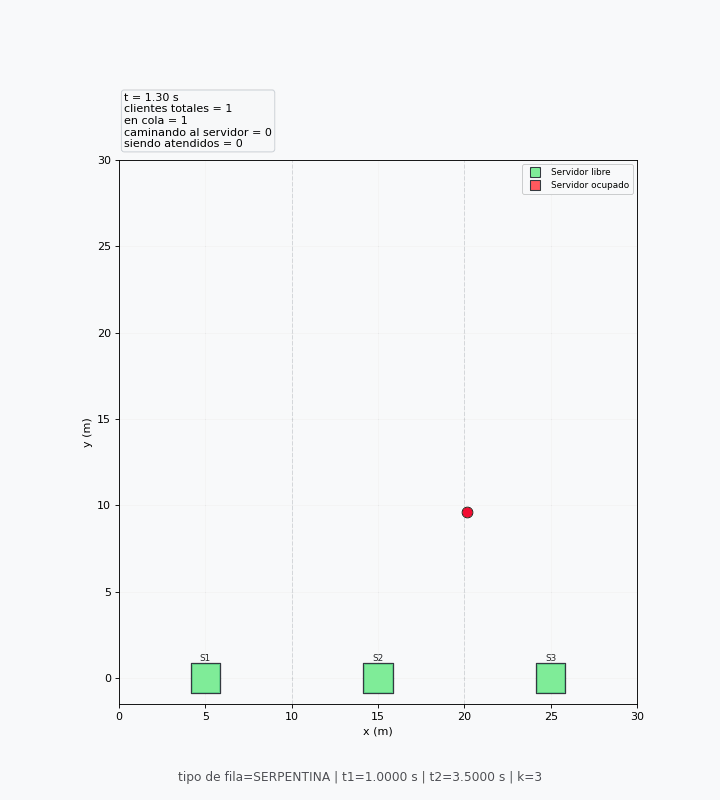
\includegraphics[height=0.42\textheight, keepaspectratio]{frame_A_SERPENTINA.png}\\[0.05cm]
        \scriptsize \texttt{Link a video: pendiente}
    \end{minipage}
    \hfill
    \begin{minipage}[t]{0.48\textwidth}
        \centering
        \small Fila libre\\[0.1cm]
        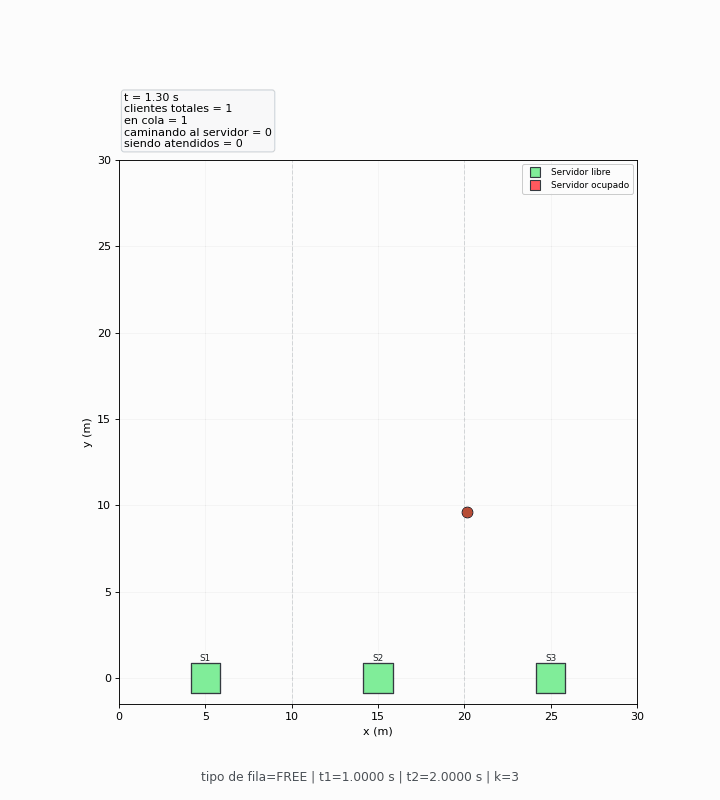
\includegraphics[height=0.42\textheight, keepaspectratio]{frame_A_FREE.png}\\[0.05cm]
        \scriptsize \url{https://youtube.com/shorts/uP6HpX2jsdU?feature=share}
    \end{minipage}

    \vspace{0.15cm}
    \paramsbox{Ejemplos ilustrativos con modalidad A y $k=3$.}
\end{frame}

\begin{frame}{Barrido de $t_2$}{Modalidad A}
    \resultpair
        {Largo promedio de fila}
        {1_input-t2/1_sweep_A_SERPENTINA_largo_fila.png}
        {Tasa de crecimiento}
        {1_input-t2/1_sweep_A_SERPENTINA_tasa_crecimiento.png}
        {$t_1 = 1\,\mathrm{s}$ | $k = 5$ | fila guiada: serpentina | $t_f = 1000\,\mathrm{s}$}
\end{frame}

\begin{frame}{Barrido de $t_2$}{Modalidad A}
    \resultpair
        {Histograma de permanencia, $t_2 = 1\,\mathrm{s}$}
        {1_input-t2/2_sweep_A_SERPENTINA_hist_permanencia_t2=1.png}
        {Histograma de permanencia, $t_2 = 4\,\mathrm{s}$}
        {1_input-t2/2_sweep_A_SERPENTINA_hist_permanencia_t2=4.png}
        {$t_1 = 1\,\mathrm{s}$ | $k = 5$ | fila guiada: serpentina | $t_f = 1000\,\mathrm{s}$}
\end{frame}

\begin{frame}{Barrido de $t_2$}{Modalidad A}
    \resultpair
        {Histograma de permanencia, $t_2 = 8\,\mathrm{s}$}
        {1_input-t2/2_sweep_A_SERPENTINA_hist_permanencia_t2=8.png}
        {Permanencia promedio}
        {1_input-t2/3_sweep_A_SERPENTINA_permanencia.png}
        {$t_1 = 1\,\mathrm{s}$ | $k = 5$ | fila guiada: serpentina | $t_f = 1000\,\mathrm{s}$}
\end{frame}

\begin{frame}{Barrido de $t_2$}{Modalidad B}
    \resultpair
        {Largo promedio de fila}
        {1_input-t2/4_sweep_B_SERPENTINA_largo_fila.png}
        {Tasa de crecimiento}
        {1_input-t2/4_sweep_B_SERPENTINA_tasa_crecimiento.png}
        {$t_1 = 1\,\mathrm{s}$ | $k = 5$ | fila guiada: serpentina | $t_f = 1000\,\mathrm{s}$}
\end{frame}

\begin{frame}{Barrido de $t_2$}{Modalidad B}
    \resultpair
        {Histograma de permanencia, $t_2 = 1\,\mathrm{s}$}
        {1_input-t2/5_sweep_B_SERPENTINA_hist_permanencia_t2=1.png}
        {Histograma de permanencia, $t_2 = 4\,\mathrm{s}$}
        {1_input-t2/5_sweep_B_SERPENTINA_hist_permanencia_t2=4.png}
        {$t_1 = 1\,\mathrm{s}$ | $k = 5$ | fila guiada: serpentina | $t_f = 1000\,\mathrm{s}$}
\end{frame}

\begin{frame}{Barrido de $t_2$}{Modalidad B}
    \resultpair
        {Histograma de permanencia, $t_2 = 8\,\mathrm{s}$}
        {1_input-t2/5_sweep_B_SERPENTINA_hist_permanencia_t2=8.png}
        {Permanencia promedio}
        {1_input-t2/6_sweep_B_SERPENTINA_permanencia.png}
        {$t_1 = 1\,\mathrm{s}$ | $k = 5$ | fila guiada: serpentina | $t_f = 1000\,\mathrm{s}$}
\end{frame}

\begin{frame}{Barrido de $t_2$}{Comparaci\'on entre modalidades}
    \resultpair
        {Histograma de permanencia, $t_2 = 3\,\mathrm{s}$}
        {1_input-t2/7_sweep_AvB_t2_SERPENTINA_hist_permanencia_t2=3.png}
        {Largo promedio de fila}
        {1_input-t2/7_sweep_AvB_t2_SERPENTINA_largo_fila.png}
        {$t_1 = 1\,\mathrm{s}$ | $k = 5$ | fila guiada: serpentina | $t_f = 1000\,\mathrm{s}$}
\end{frame}

\begin{frame}{Barrido de $t_1$}{Modalidad A}
    \resultpair
        {Largo promedio de fila}
        {2_input-t1/1_sweep_A_t1_SERPENTINA_largo_fila.png}
        {Tasa de crecimiento}
        {2_input-t1/1_sweep_A_t1_SERPENTINA_tasa_crecimiento.png}
        {$t_2 = 3\,\mathrm{s}$ | $k = 5$ | fila guiada: serpentina | $t_f = 1000\,\mathrm{s}$}
\end{frame}

\begin{frame}{Barrido de $t_1$}{Modalidad A}
    \resultpair
        {Histograma de permanencia, $t_1 = 0.3\,\mathrm{s}$}
        {2_input-t1/2_sweep_A_t1_SERPENTINA_hist_permanencia_t1=0.3.png}
        {Histograma de permanencia, $t_1 = 1.8\,\mathrm{s}$}
        {2_input-t1/2_sweep_A_t1_SERPENTINA_hist_permanencia_t1=1.8.png}
        {$t_2 = 3\,\mathrm{s}$ | $k = 5$ | fila guiada: serpentina | $t_f = 1000\,\mathrm{s}$}
\end{frame}

\begin{frame}{Barrido de $t_1$}{Modalidad A}
    \resultpair
        {Histograma de permanencia, $t_1 = 3\,\mathrm{s}$}
        {2_input-t1/2_sweep_A_t1_SERPENTINA_hist_permanencia_t1=3.png}
        {Permanencia promedio}
        {2_input-t1/3_sweep_A_t1_SERPENTINA_permanencia.png}
        {$t_2 = 3\,\mathrm{s}$ | $k = 5$ | fila guiada: serpentina | $t_f = 1000\,\mathrm{s}$}
\end{frame}

\begin{frame}{Barrido de $t_1$}{Modalidad B}
    \resultpair
        {Largo promedio de fila}
        {2_input-t1/4_sweep_B_t1_SERPENTINA_largo_fila.png}
        {Tasa de crecimiento}
        {2_input-t1/4_sweep_B_t1_SERPENTINA_tasa_crecimiento.png}
        {$t_2 = 3\,\mathrm{s}$ | $k = 5$ | fila guiada: serpentina | $t_f = 1000\,\mathrm{s}$}
\end{frame}

\begin{frame}{Barrido de $t_1$}{Modalidad B}
    \resultpair
        {Histograma de permanencia, $t_1 = 0.3\,\mathrm{s}$}
        {2_input-t1/5_sweep_B_t1_SERPENTINA_hist_permanencia_t1=0.3.png}
        {Histograma de permanencia, $t_1 = 1.8\,\mathrm{s}$}
        {2_input-t1/5_sweep_B_t1_SERPENTINA_hist_permanencia_t1=1.8.png}
        {$t_2 = 3\,\mathrm{s}$ | $k = 5$ | fila guiada: serpentina | $t_f = 1000\,\mathrm{s}$}
\end{frame}

\begin{frame}{Barrido de $t_1$}{Modalidad B}
    \resultpair
        {Histograma de permanencia, $t_1 = 3\,\mathrm{s}$}
        {2_input-t1/5_sweep_B_t1_SERPENTINA_hist_permanencia_t1=3.png}
        {Permanencia promedio}
        {2_input-t1/6_sweep_B_t1_SERPENTINA_permanencia.png}
        {$t_2 = 3\,\mathrm{s}$ | $k = 5$ | fila guiada: serpentina | $t_f = 1000\,\mathrm{s}$}
\end{frame}

\begin{frame}{Barrido de $t_1$}{Comparaci\'on entre modalidades}
    \resultpair
        {Histograma de permanencia, $t_1 = 3\,\mathrm{s}$}
        {2_input-t1/7_sweep_AvB_t1_SERPENTINA_hist_permanencia_t1=3.png}
        {Largo promedio de fila}
        {2_input-t1/7_sweep_AvB_t1_SERPENTINA_largo_fila.png}
        {$t_2 = 3\,\mathrm{s}$ | $k = 5$ | fila guiada: serpentina | $t_f = 1000\,\mathrm{s}$}
\end{frame}

\begin{frame}{Barrido de $k$}{Modalidad A}
    \resultpair
        {Largo promedio de fila}
        {3_input-k/1_sweep_A_k_SERPENTINA_largo_fila.png}
        {Tasa de crecimiento}
        {3_input-k/1_sweep_A_k_SERPENTINA_tasa_crecimiento.png}
        {$t_1 = 1\,\mathrm{s}$ | $t_2 = 3\,\mathrm{s}$ | fila guiada: serpentina | $t_f = 1000\,\mathrm{s}$}
\end{frame}

\begin{frame}{Barrido de $k$}{Modalidad A}
    \resultpair
        {Histograma de permanencia, $k = 1$}
        {3_input-k/2_sweep_A_k_SERPENTINA_hist_permanencia_k=1.png}
        {Histograma de permanencia, $k = 4$}
        {3_input-k/2_sweep_A_k_SERPENTINA_hist_permanencia_k=4.png}
        {$t_1 = 1\,\mathrm{s}$ | $t_2 = 3\,\mathrm{s}$ | fila guiada: serpentina | $t_f = 1000\,\mathrm{s}$}
\end{frame}

\begin{frame}{Barrido de $k$}{Modalidad A}
    \resultpair
        {Histograma de permanencia, $k = 8$}
        {3_input-k/2_sweep_A_k_SERPENTINA_hist_permanencia_k=8.png}
        {Permanencia promedio}
        {3_input-k/3_sweep_A_k_SERPENTINA_permanencia.png}
        {$t_1 = 1\,\mathrm{s}$ | $t_2 = 3\,\mathrm{s}$ | fila guiada: serpentina | $t_f = 1000\,\mathrm{s}$}
\end{frame}

\begin{frame}{Barrido de $k$}{Modalidad B}
    \resultpair
        {Largo promedio de fila}
        {3_input-k/4_sweep_B_k_SERPENTINA_largo_fila.png}
        {Tasa de crecimiento}
        {3_input-k/4_sweep_B_k_SERPENTINA_tasa_crecimiento.png}
        {$t_1 = 1\,\mathrm{s}$ | $t_2 = 3\,\mathrm{s}$ | fila guiada: serpentina | $t_f = 1000\,\mathrm{s}$}
\end{frame}

\begin{frame}{Barrido de $k$}{Modalidad B}
    \resultpair
        {Histograma de permanencia, $k = 1$}
        {3_input-k/5_sweep_B_k_SERPENTINA_hist_permanencia_k=1.png}
        {Histograma de permanencia, $k = 4$}
        {3_input-k/5_sweep_B_k_SERPENTINA_hist_permanencia_k=4.png}
        {$t_1 = 1\,\mathrm{s}$ | $t_2 = 3\,\mathrm{s}$ | fila guiada: serpentina | $t_f = 1000\,\mathrm{s}$}
\end{frame}

\begin{frame}{Barrido de $k$}{Modalidad B}
    \resultpair
        {Histograma de permanencia, $k = 8$}
        {3_input-k/5_sweep_B_k_SERPENTINA_hist_permanencia_k=8.png}
        {Permanencia promedio}
        {3_input-k/6_sweep_B_k_SERPENTINA_permanencia.png}
        {$t_1 = 1\,\mathrm{s}$ | $t_2 = 3\,\mathrm{s}$ | fila guiada: serpentina | $t_f = 1000\,\mathrm{s}$}
\end{frame}

\begin{frame}{Barrido de $k$}{Comparaci\'on entre modalidades}
    \resultpair
        {Histograma de permanencia, $k = 8$}
        {3_input-k/7_sweep_AvB_k_SERPENTINA_hist_permanencia_k=8.png}
        {Largo promedio de fila}
        {3_input-k/7_sweep_AvB_k_SERPENTINA_largo_fila.png}
        {$t_1 = 1\,\mathrm{s}$ | $t_2 = 3\,\mathrm{s}$ | fila guiada: serpentina | $t_f = 1000\,\mathrm{s}$}
\end{frame}

\section{Conclusiones}

\begin{frame}{Conclusiones}
    \begin{itemize}
        \item Para la fila guiada tipo serpentina, la modalidad A presenta menores largos de fila y menores tiempos de permanencia que la modalidad B en los tres barridos analizados.
        \item Al aumentar $t_2$, la congesti\'on y la permanencia crecen en ambas modalidades; en B la tasa de crecimiento permanece positiva en todo el rango mostrado.
        \item Al aumentar $t_1$, ambas modalidades reducen la congesti\'on, pero A alcanza valores cercanos a cero para largos de fila m\'as r\'apidamente que B.
        \item Al aumentar $k$, ambas modalidades mejoran, aunque la reducci\'on de cola y permanencia es mucho m\'as marcada en A que en B.
    \end{itemize}
\end{frame}

\begin{frame}
    \begin{beamercolorbox}[sep=8pt,center]{title}
        \usebeamerfont{title} Muchas gracias
    \end{beamercolorbox}
\end{frame}

\end{document}
